\section{Network Characteristics of OS Services}
\label{sec:characterize-os}

Mobile operating systems provide APIs and OS level services to optimize network usage.
For example, the Apple Push Notification service (APNs) and Google Cloud Messaging (GCM)~\cite{gcm} are used by iOS applications and Android applications respectively to receive notifications from the Internet.
In this section we present the results of our controlled experiments and measurements performed in the wild to detail the network characteristics of these OS services.
The questions that we answer in this section are as follows.
\begin{packedenumerate}
\item What are the network characteristics of operating system services?
\item How different is the network traffic from iOS devices compared to Android devices?
\item What is the impact of operating system services in the wild?
\end{packedenumerate}

\subsection{Controlled Experiment on Factory Reset Devices}

We performed a controlled experiment to detail the network characteristics of mobile devices and the pre-installed applications.
The objective of this experiment was to answer the following questions.
\begin{packedenumerate}
\item What is the network usage of devices that are used \emph{out of the box}? 
\item How does the device, manufacturer, and operating system affect the network usage?
\end{packedenumerate}

For our experiment, we performed a \emph{factory reset} on an iPod Touch, an iPad, an iPhone, a Samsung Galaxy SIII, and a Google Nexus S Phone.
Each of these devices were reset to factory default settings after their batteries were fully charged. 
We then allowed these devices to connect to the Internet over \wifi through \platname and monitored the Internet traffic from these devices for 3 sessions of 24 hours. 
To compare the impact of access technology we let the iPhone and Samsung Galaxy SIII connected tunnel traffic through \platname using cellular networks. 
During the initialization, we assigned a dummy email account as the primary account to each of these devices; we observed devices exchanged from 20 MB to 50 MB during initialization. 

We observed that the traffic volume during the 24 hour periods varied from 19~KB to 97~KB depending on the devices. 
We classify APNS and GCM messages using the TCP port numbers mentioned in their specifications~\cite{gcm, apns}.
Based on this classification we observe that share of push notifications varied from 35\% to 88\% of the total traffic volume during the 24 hour interval. 
The share of DNS traffic varied from 10\% to 40\% for each of the devices while the other services contributed to less than 10\% of the traffic volume.
The only exception was the Samsumg Galaxy SIII which used location services that contributed to 26\% of 47~KB traffic volume.

\begin{figure}
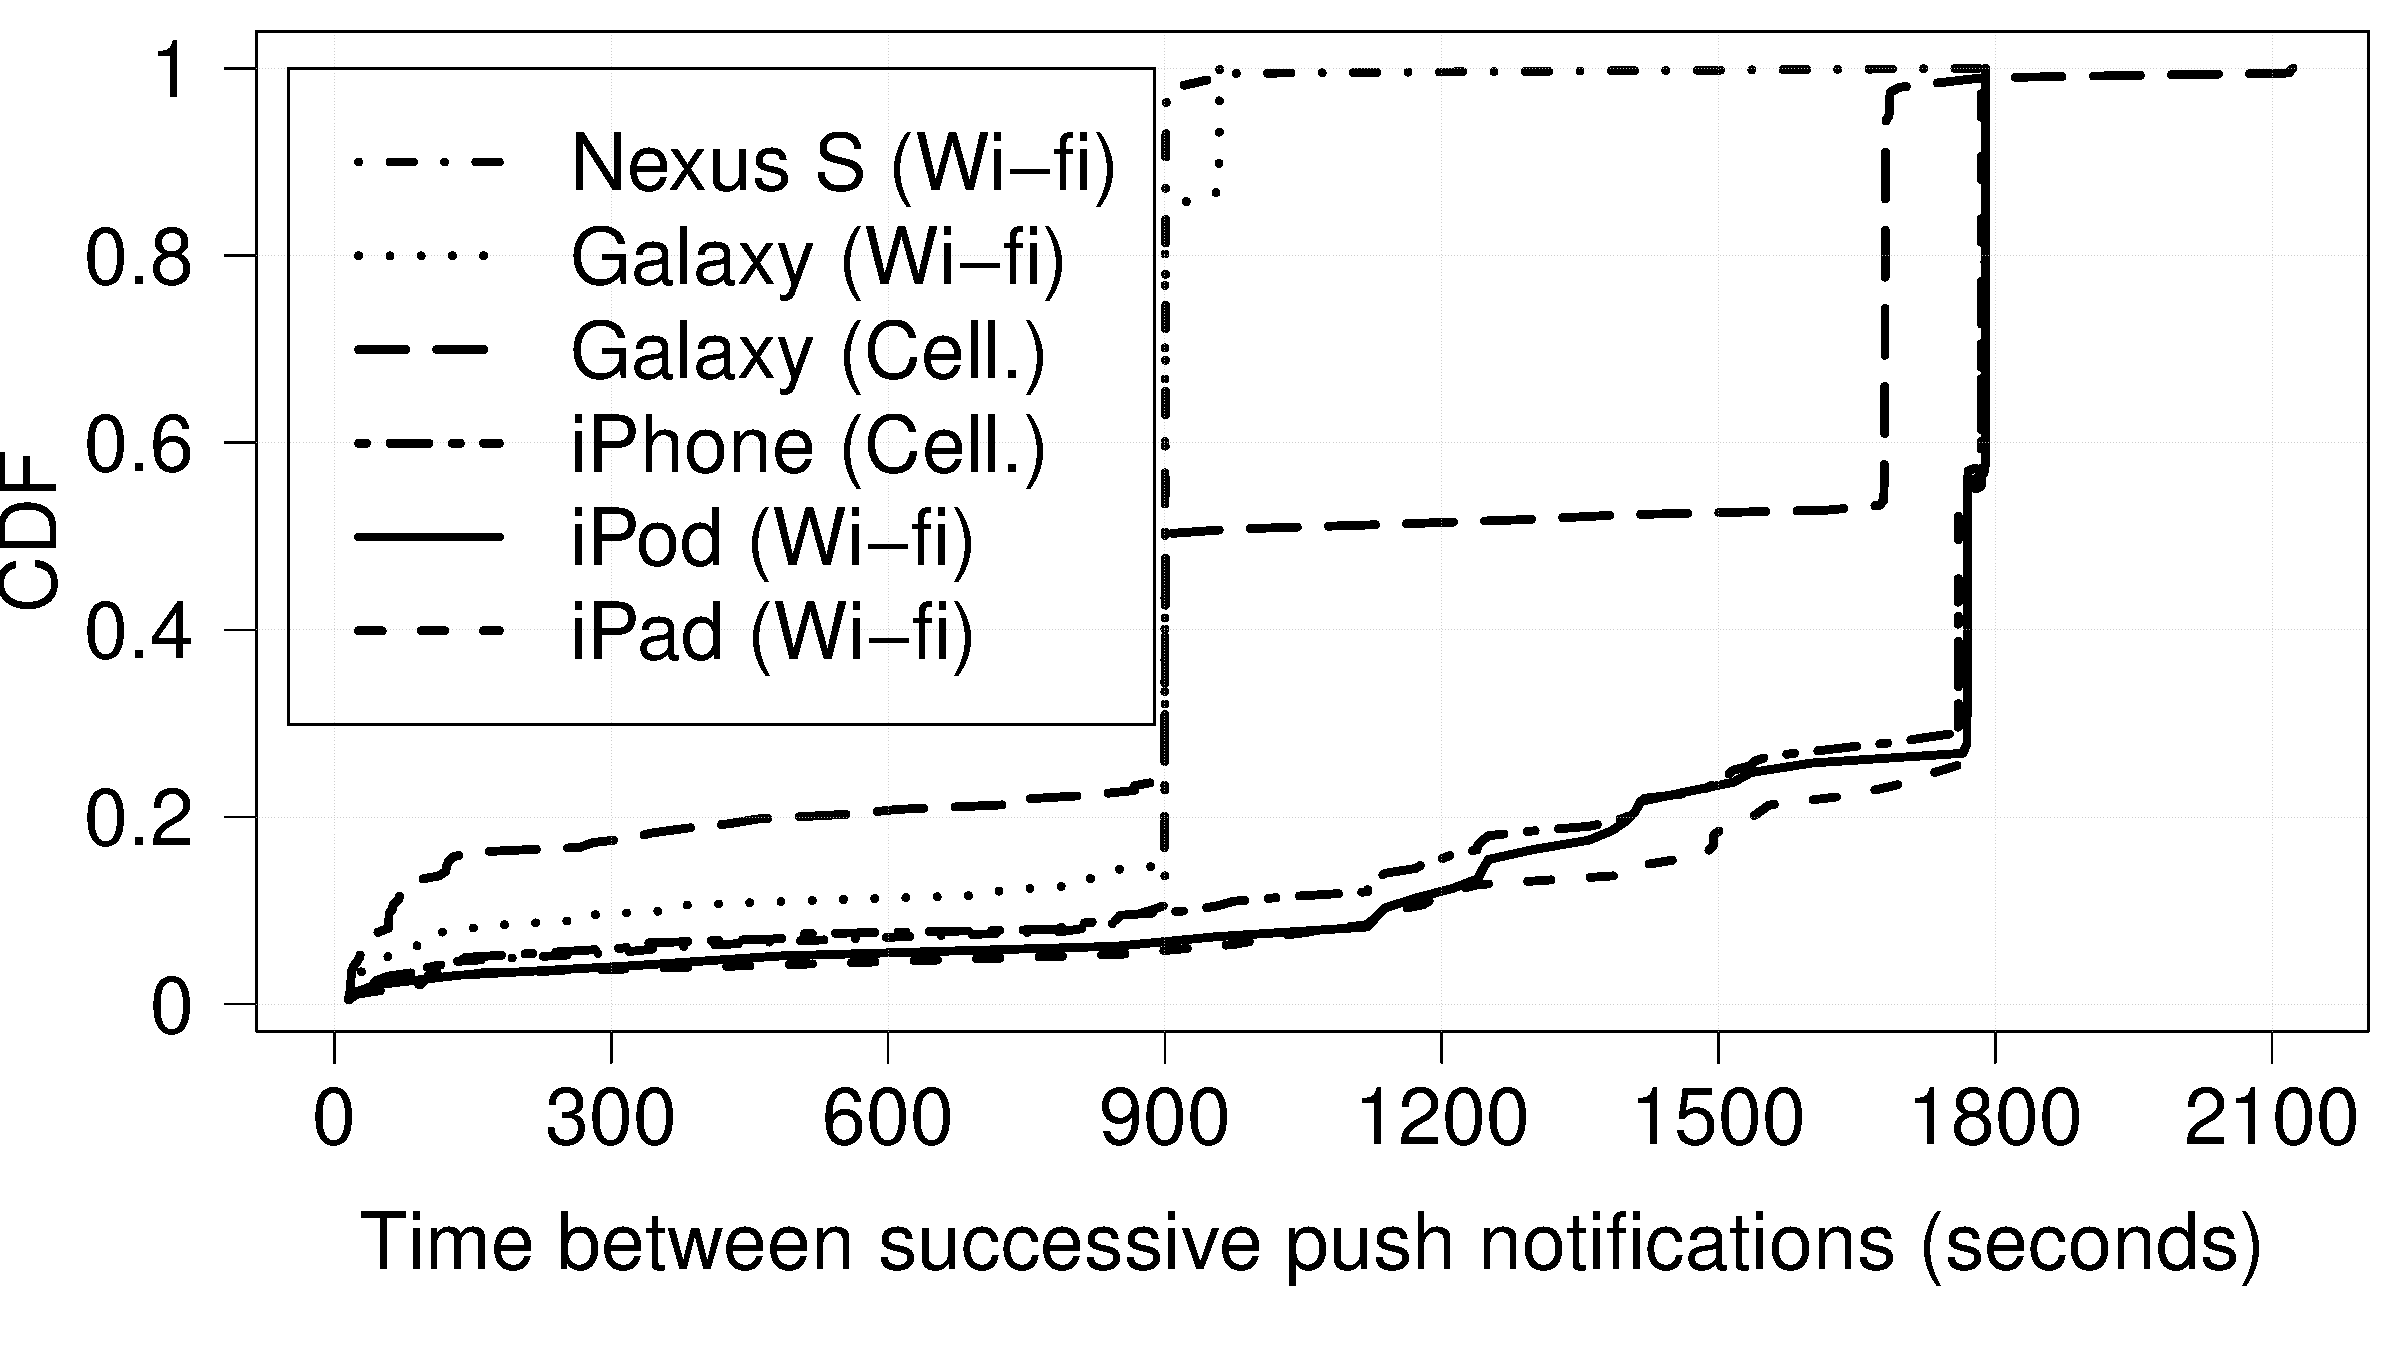
\includegraphics[width=\columnwidth]{plots/push_inter_arrival.pdf}
\caption{Inter-arrival time between push notification messages after factory reset. \emph{The Android and iOS devices communicate with the notification server approximately once every 900~seconds and 1800 seconds respectively. The behavior of Android devices depends on the device and the pre-installed applications.}}
\label{fig:inter-arrival-push}
\end{figure}

In \fref{fig:inter-arrival-push} we plot the time between successive messages exchanged on the ports used for push notifications. 
We observe that the inter-arrival time between push notifications for the Android devices is at least 900 seconds for more than 80\% of the push notifications observed. 
The distribution of the inter-arrival time also depends on the access technology for the Samsung Galaxy SIII phone; we observe steps in the distribution at 900 seconds, 1680~seconds, and 2110 seconds when the device uses cellular connection. 
We do not observe this difference for the Nexus S phone; we do not present the figure due to lack of space. 
\tbd{Why these difference -- which applications stop coming up and so on}.
For the iOS devices, we observe an inter-arrival time at least 1700~seconds for that more than 75\% of the push notifications. 
We do not observe a significant difference between the inter-arrival times for the iPhone over cell and \wifi and we do not present these results due to lack of space. 
All Android flows with an inter-arrival time larger than 800 seconds consisted of an empty TCP packet sent by the device followed by a 25 byte payload sent by the server.
All iOS flows with an inter-arrival time larger than 1500 seconds began with an TCP packet with a payload of 85 bytes sent by the device followed by the server responding with of a TCP packet of 37 byte payload.


In summary, we observe push notifications for Android devices and iOS devices are have a very small footprint in terms of data consumption in the default state.
The iOS devices have a larger time between successive push notifications compared to Android devices in the default state. 
Furthermore, the inter-arrival time between push notifications for Android devices differs based on the manufacturer and the access technology.

\tbd{power impact}

\subsection{Push Notifications In The Wild} 

We now characterize our observations on the push notifications we observed in the \mobWild dataset. 
The objective of this analysis was to answer the following questions
\begin{packedenumerate}
\item How frequently do Push notifications take place in the wild?
\item What is the impact of access technology on push notifications?
\item \tbd{What is the distribution of traffic volume of push notifications?}	
\item \tbd{How do push notifications change over OS and device upgrades?}
\item \tbd{Do not disturb -- How efficient are services like Do Not Disturb?}
\end{packedenumerate}

\begin{figure}
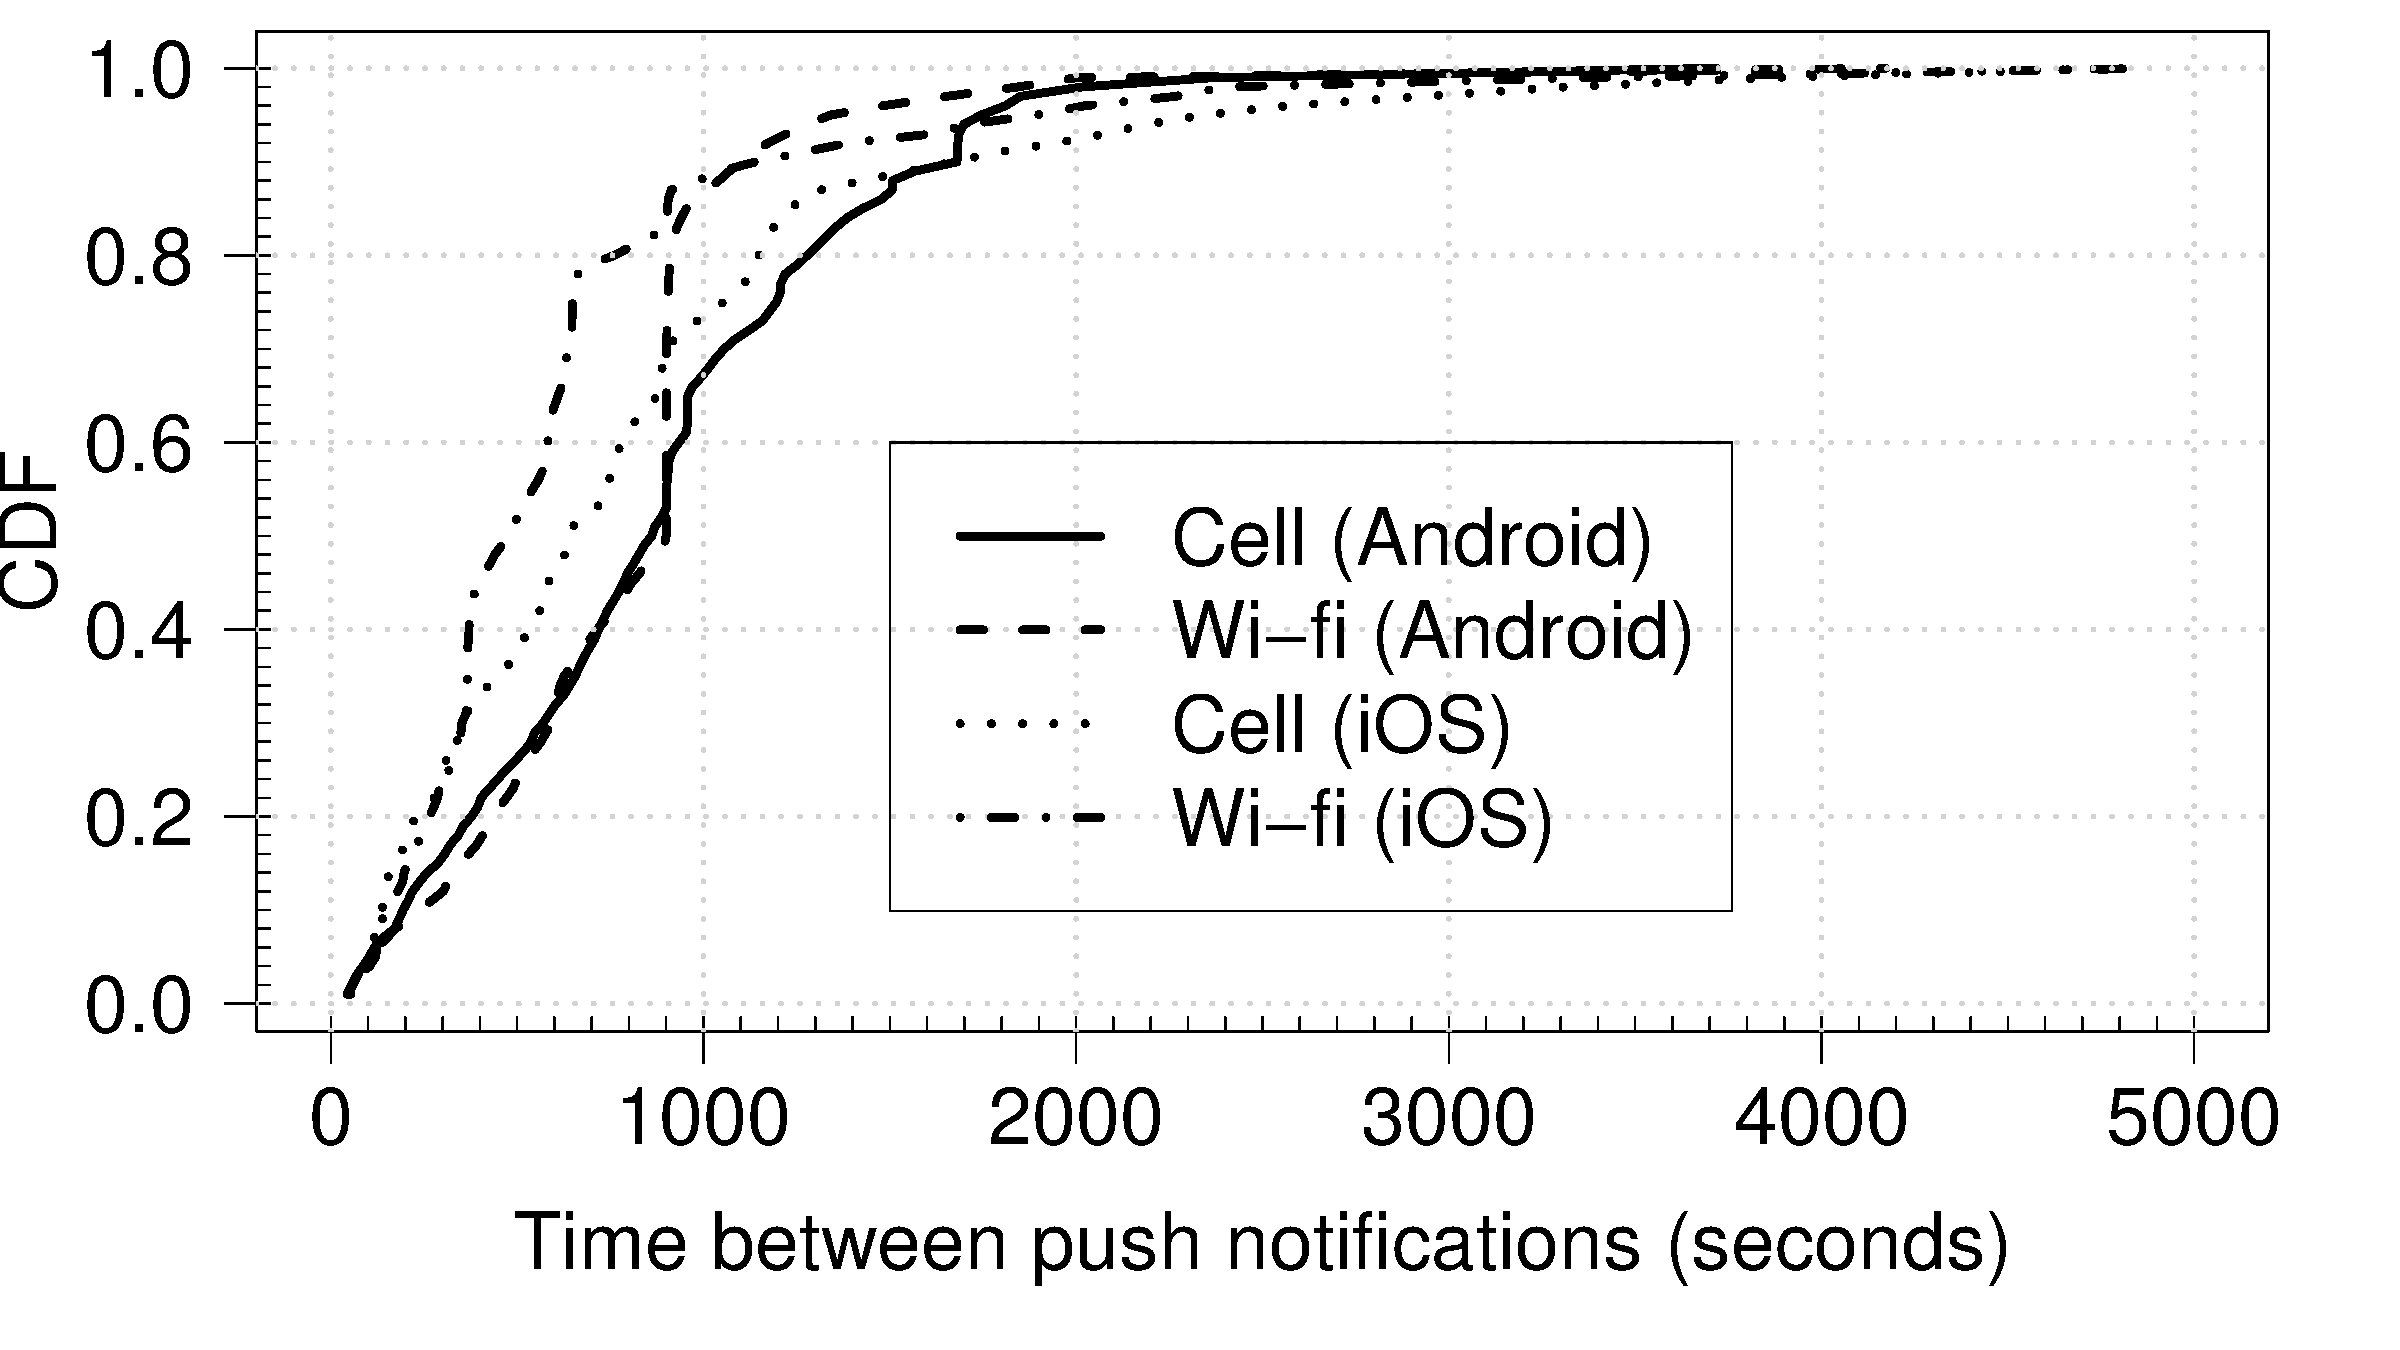
\includegraphics[width=\columnwidth]{plots/cdf_push_comparison_device_wild.pdf}
\caption{Distribution of the time between push notification messages in the wild. \emph{The frequency of push notification messages is higher for the iOS devices in our dataset compared to the Android devices. Notification messages are less frequent over cellular networks compared to Wi-Fi networks.}}
\label{fig:wild-cdf-push}
\end{figure}

%The advantage of \platname is that it allows for direct comparison between devices across and their behavior across access technologies. 
In \fref{fig:wild-cdf-push} we plot the distribution of the time between successive push notification messages for Android and iOS devices over cellular and \wifi networks. 
While computing this distribution, we account the diversity in device usage in the following manner.
For each device and each access technology we compute the 100 quantiles from 0.01 to 1.0 in steps of 0.01 of the time between successive push notifications. 
We then use the median value of each quantile (from 0.01 to 1.0 in steps of 0.01) for a given access technology and operating system of the device.
In \ref{fig:inter-arrival-push} we observe a higher time between push notifications on cellular networks compared to \wifi networks. 
We also observe that the time between push notifications is higher for the iOS devices in our dataset compared to the Android devices in our dataset. 
\tbd{The tcp ports used after the push notifications. Numbers for what fraction was ssl traffic at 443. and the servers to which the connection was made.}

\begin{figure}
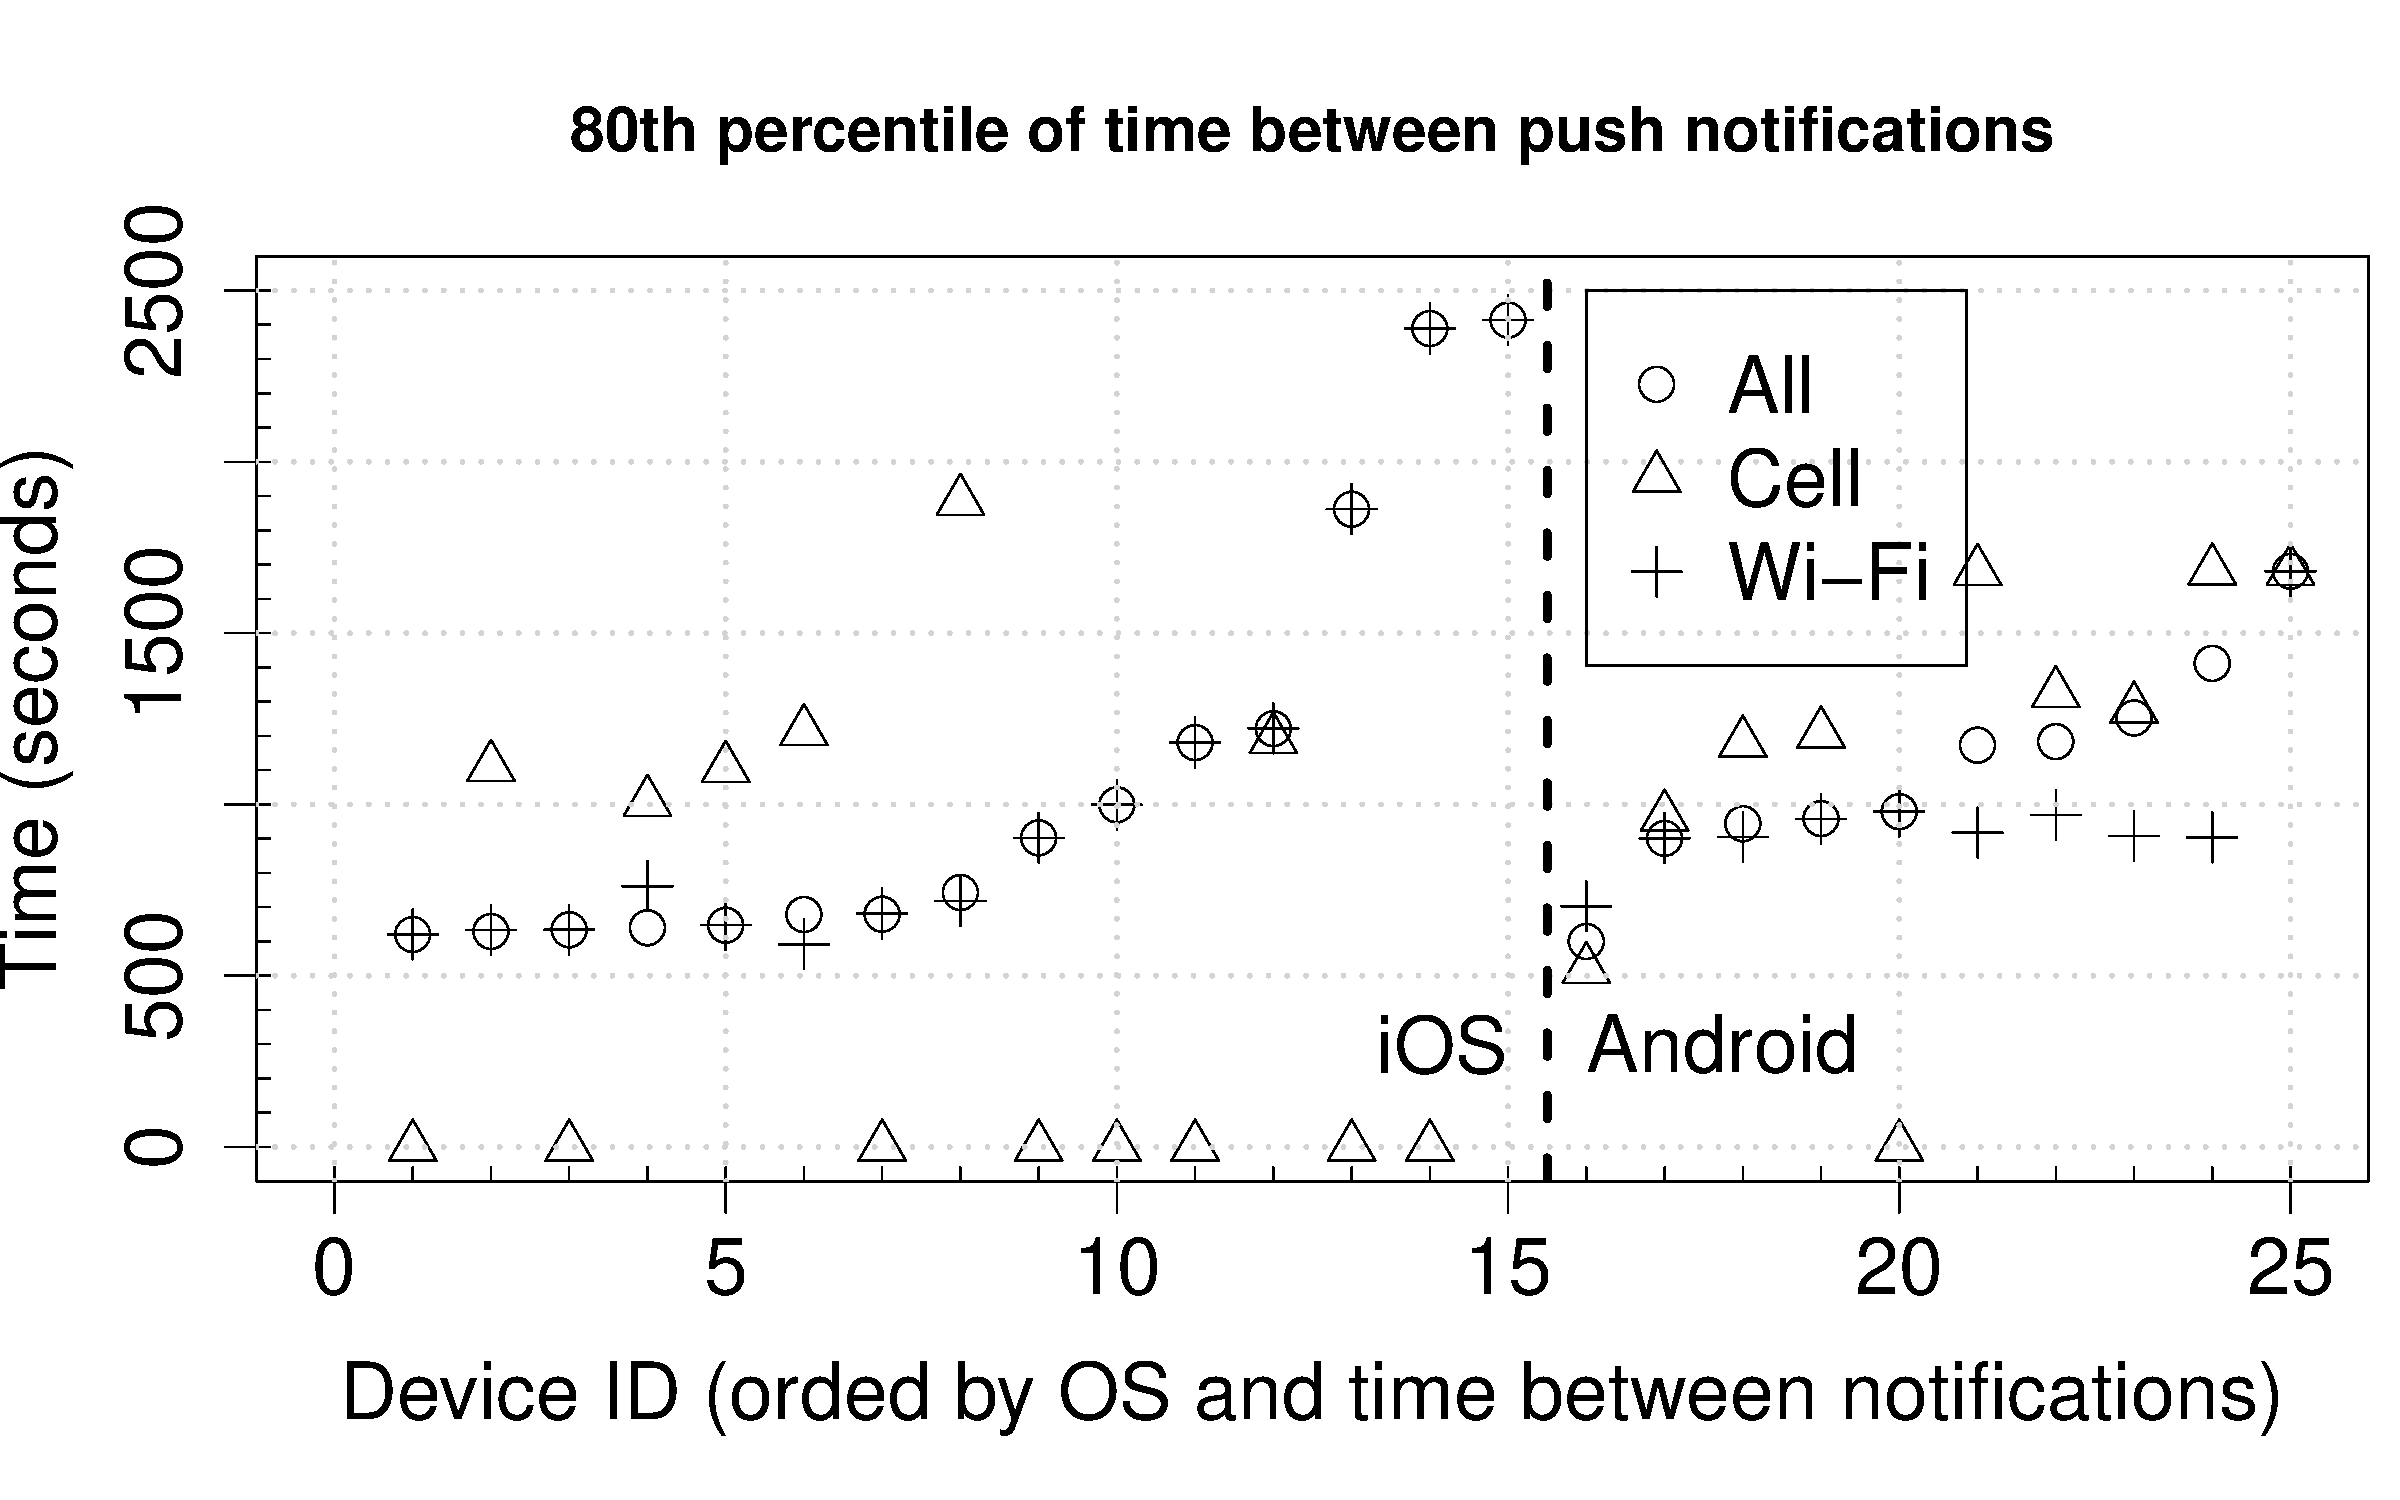
\includegraphics[width=\columnwidth]{plots/push_inter_arrival_wild.pdf}
\caption{Inter-arrival time between push notifications in the wild. \emph{Push notifications occur less frequently over Cellular networks. The rate of push notifications depends on users and the applications installed. \tbd{DISCUSS: Better representation for tablets -- currently they have a value of 0 for the cell networks.}}}
\label{fig:wild-inter-arrival-push}
\end{figure}


In \fref{fig:wild-inter-arrival-push} we present the time between successive push notifications for the 25 devices in our dataset. 
As observed in \fref{fig:wild-cdf-push} we observe that the iOS devices receive push messages more frequently that the Android devices. 
We also observe that the time between push notifications is higher for Android devices.
The iOS devices prefer a cellular data connection for Push notification over \wifi \tbd{http://support.apple.com/kb/TS4264}. 
However, in \fref{fig:wild-cdf-push} and \fref{fig:wild-cdf-push} despite this preference, we observe that the time between successive push notifications for iOS devices is higher over cellular networks in comparison to \wifi networks.  
We observe that \tbd{SSL traffic} to mail servers was followed \tbd{x\%} after push notifications.
This implies that higher usage of the device over \wifi may result in a higher number of notificatons received. 
In \fref{fig:wild-inter-arrival-push}, device ID 
%Only if the cellular connection is not available or viable will the device switch to Wi-Fi for APNs connections.


\begin{figure}
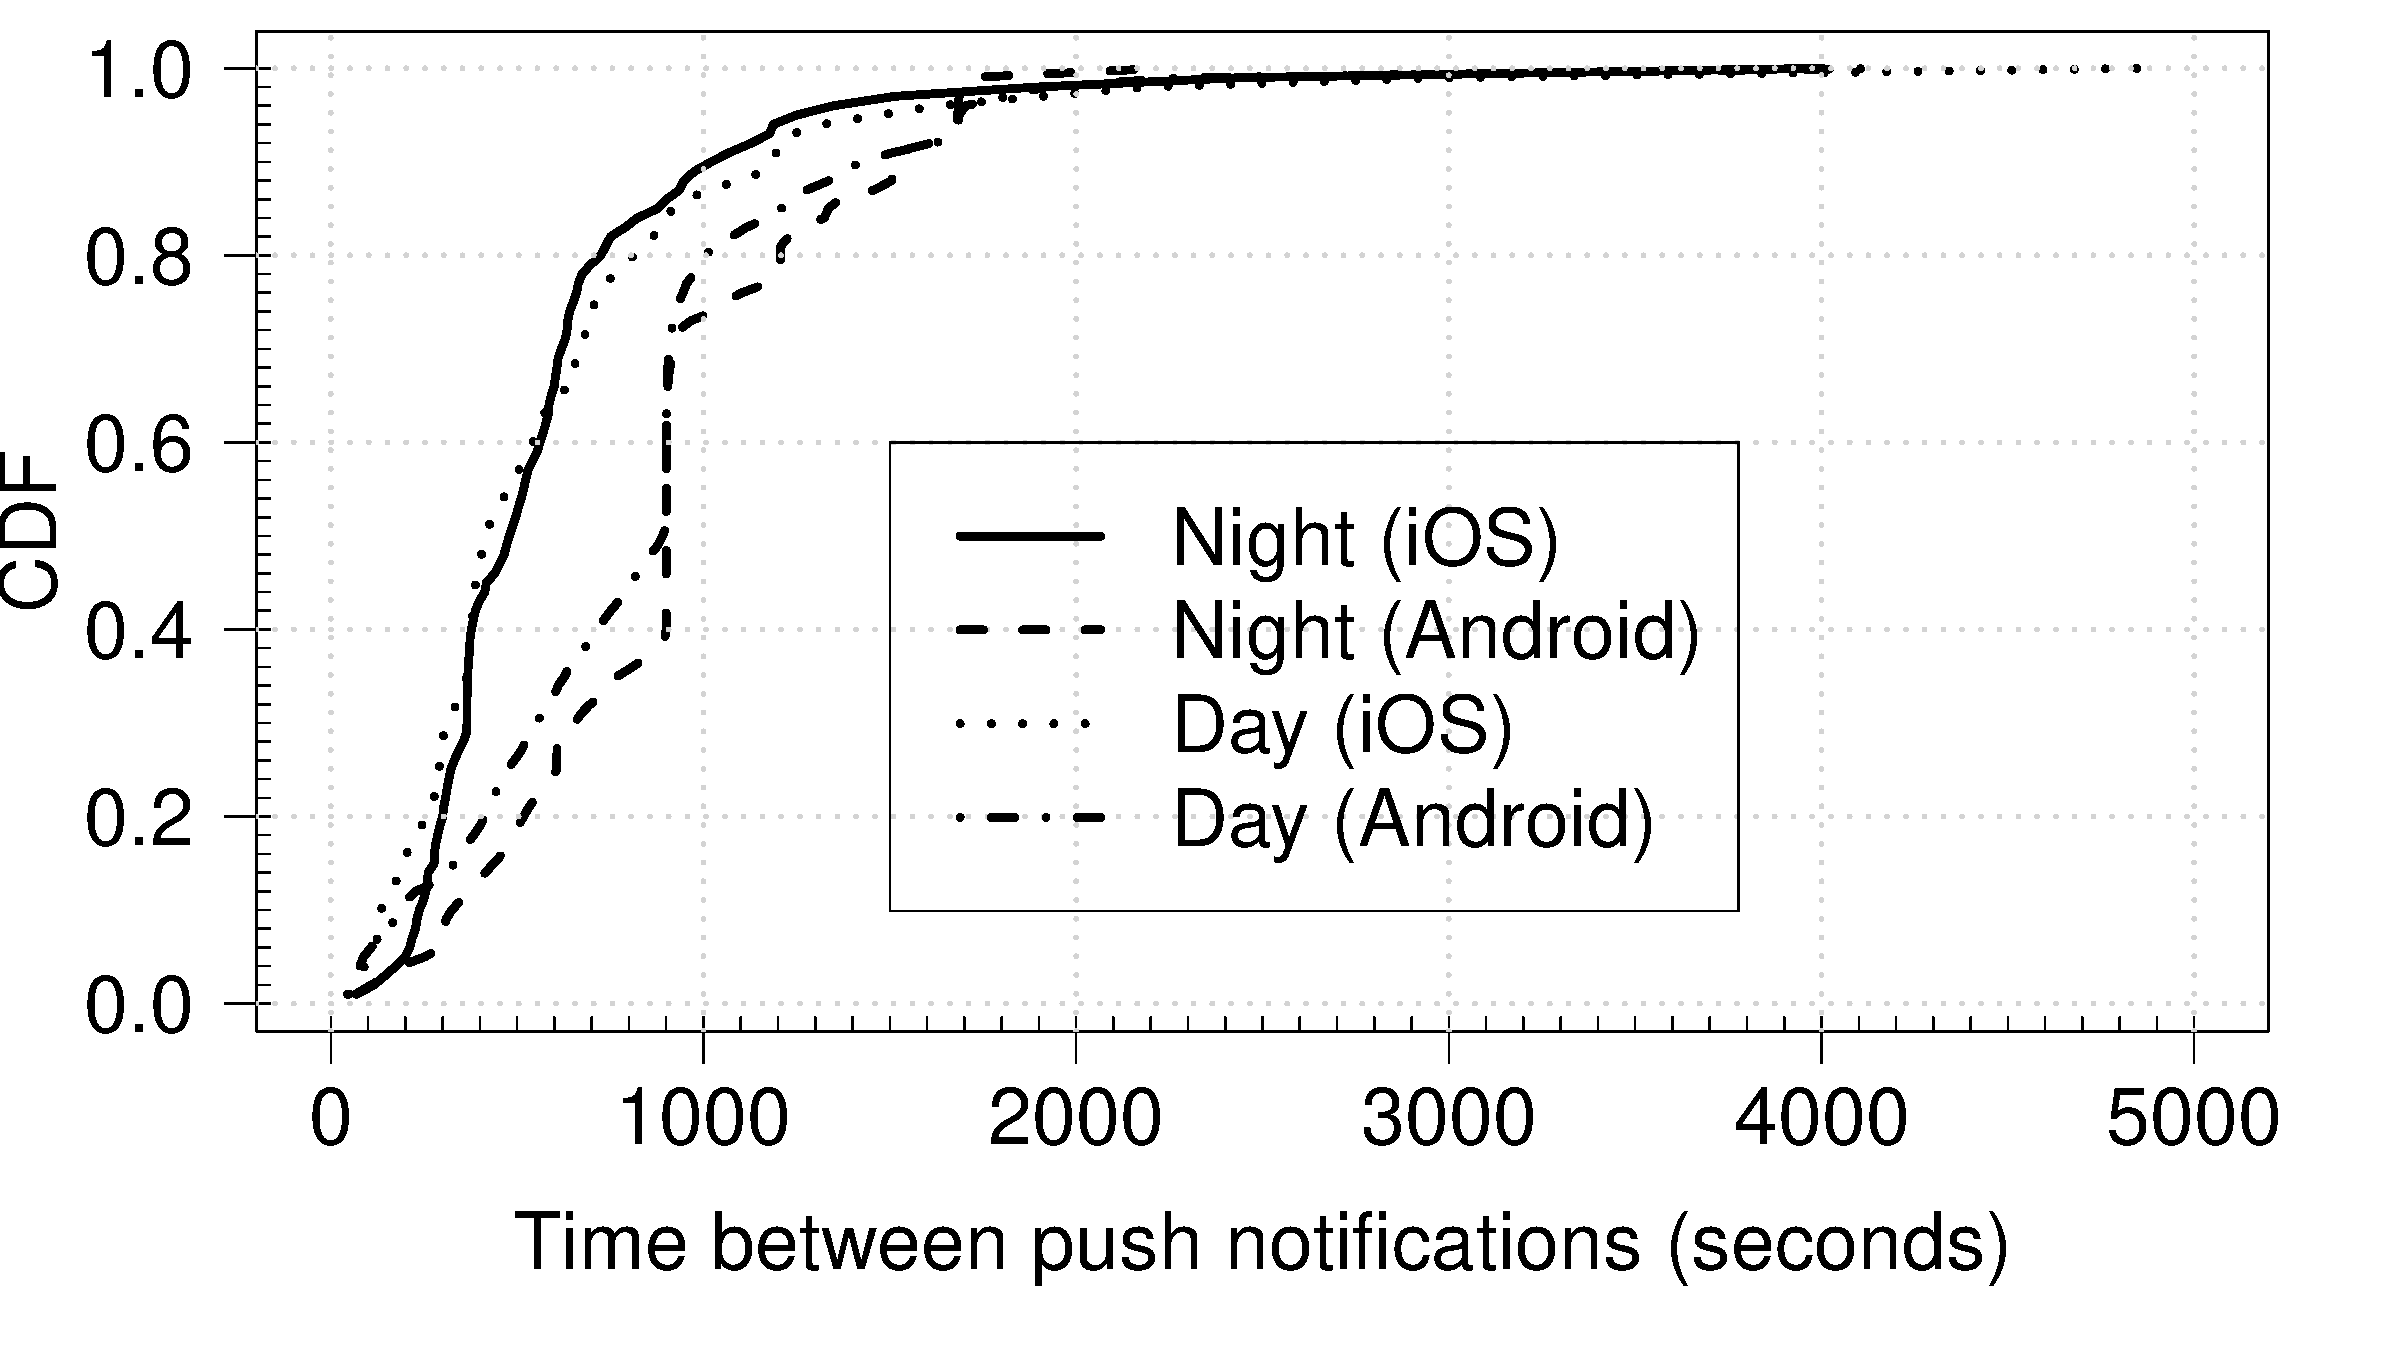
\includegraphics[width=\columnwidth]{plots/cdf_night_push_comparison_device_wild.pdf}
\caption{Impact of time-of-day on the push notifications. \emph{The rate of push notifications is agnostic of the time of the day for iOS devices.}}
\label{fig:wild-cdf-push-night}
\end{figure}

\tbd{Highlight the pervasive nature of \platname  allows us}
We now use \fref{fig:wild-cdf-push-night} we to show that the push notification are agnostic of the time of the day. 
For \fref{fig:wild-cdf-push-night}, we consider two time periods: from midnight to 6 am (\emph{Night}) and from 6 am to midnight (\emph{Day}).
The values used in the distributions is computed using the technique used for \ref{fig:wild-cdf-push}. 
We observe that the Android and iOS devices exhibit a similar behavior that appears to be agnostic of the time of the day. 
The iOS devices (from verion 6.0) come with a feature called \emph{Do Not Disturb (DND)} that does raise notification alarms on receiving notifications during specific time periods. 
We also observe that during the intervals configured as \emph{Do Not Disturb}, notification messages were exchanged by devices that used this feature enabled. 

\tbd{Who is pushing the notifications. Servers used for push notifications..based on DNS requests responses}


%\subsection{Discussion}




% OLD TABLE WITHOUT IPHONE
% \begin{table}
% \begin{small}
% \begin{tabular}{|c|c|c|c|c|}
% \hline
% \multirow{2}{*}{\bf Application} & \multicolumn{4}{c|}{\bf Traffic Share in the first 24 hours}\tabularnewline
% \cline{2-5}
%      & iPad & iPod & Galaxy SIII & Nexus \tabularnewline
%      & (19 KB) & (21 KB) & (47 KB)& (97 KB)  \tabularnewline
% \hline
% Notifications & 0.54 & 0.53 & 0.35 & 0.88 \tabularnewline
% \hline
% Location & 0 & 0 & 0.26 & 0 \tabularnewline
% \hline
% SSL & 0 & 0 & 0.30 & 0.11 \tabularnewline
% \hline
% Mail & 0.05 & 0.07 & 0 & 0 \tabularnewline
% \hline
% HTTP & 0.13 & 0 & 0.09  & 0 \tabularnewline
% \hline
% UDP & 0.28 & 0.40 & 0.01 & 0.01 \tabularnewline
% \hline
% {\em total}& {\em 1.0} & {\em 1.0} & {\em 1.0} & {\em 1.0}\tabularnewline
% \hline
% \end{tabular}
% \end{small}
% \caption{Network usage in the first 24 hours after factory reset. \emph{Notifications contribute to the largest fraction of traffic volume across all devices.}}
% \label{tab:traffic-share-factory-reset}
% \end{table}
